\subsection{Motivation}
Climate and environmental science depend on repeat optical imaging of regions such as tropical rainforests, where cloud cover is frequent and unpredictable at the timescale of a satellite pass.
Mission operators today often rely on deterministic strategies with fixed nadir attitude and pre-planned shutter times that treat every target along a ground track equally.
When clouds occlude the line of sight, those strategies still consume onboard memory and downlink budget on low-value frames, while scientists lose observations that may not be recoverable on the next pass.
The cost is therefore threefold: reduced science yield, wasted capture capacity, and unnecessary actuator activity from indiscriminate pointing and slewing.

Autonomous onboard decision-making is motivated by latency: ground-in-the-loop replanning cannot react to the cloud layout actually present during the pass.
Both \emph{when} to expose the shutter and \emph{how} to orient the spacecraft for maximal image quality therefore matter, and they must respect attitude safety limits on reaction-wheel use and pointing envelopes.
From the outside, the required behaviour looks straightforward: use onboard camera feedback to skip cloud-occluded targets and capture only when the view is clear.
This report treats that apparent simplicity as the starting point and asks what training design is actually required to reach it.

The specific orbit geometry is not tied to a polar versus equatorial regime.
Any circular orbit viewed at the instant of overflight is equivalent for the control problem posed here.

\paragraph{Current operational process.}
In a typical Earth-observation mission today, domain scientists compile a list of target areas they wish to image and submit it to mission control.
The ground segment then builds an observation schedule: it checks which targets fall within the satellite's ground track on upcoming passes, verifies observable constraints such as solar illumination and off-nadir angle limits, and uplinks a fixed command sequence.
This process works well for constraints that can be predicted from orbital mechanics.
Cloud cover, however, cannot be scheduled out: the weather state at the moment of overflight is unknown at planning time, and the uplinked schedule cannot be modified during the pass.
The satellite therefore executes its pre-planned capture sequence regardless of what the cameras actually see, consuming onboard storage, electrical power, downlink capacity, and attitude-control effort on frames that may be entirely cloud-occluded \citep{ferrari2024ssp}.

\subsection{Intended solution concept}
\label{sec:solution-concept}

Today's operational process is ground-planned: the capture list is fixed before the pass, and uplink latency is too large for cloud-aware replanning during overflight.
Under that paradigm a forward-looking sensor has little operational value, because the satellite cannot act on what it sees ahead.
Consequently, current missions typically do not fly a dedicated lookahead imager for in-pass scheduling.

An onboard scheduling agent changes that premise.
If capture decisions are made during the pass, the agent needs information about upcoming targets and cloud conditions \emph{before} those scenes enter the primary imaging window.
Otherwise it can react only when a target is already under the science boresight, which is too late for useful opportunity selection under a limited shutter budget.

The primary payload is a narrow-field science camera (hyperspectral-class in the mission concept).
Pointing that instrument forward would still cover only a thin along-track strip, so it is a poor lookahead sensor for surveying multiple upcoming opportunities.
This study therefore adds a second, forward-tilted wide-angle (fisheye) camera that observes the corridor ahead while the primary camera remains dedicated to science capture near nadir
(Table~\ref{tab:constants-camera-sim}; $\SI{70}{\degree}$ along-track FOV, $\SI{25}{\degree}$ prograde tilt).
Figure~\ref{fig:concept-lookahead} illustrates this sensing geometry on a representative along-track pass.

\begin{figure}[htbp]
  \centering
  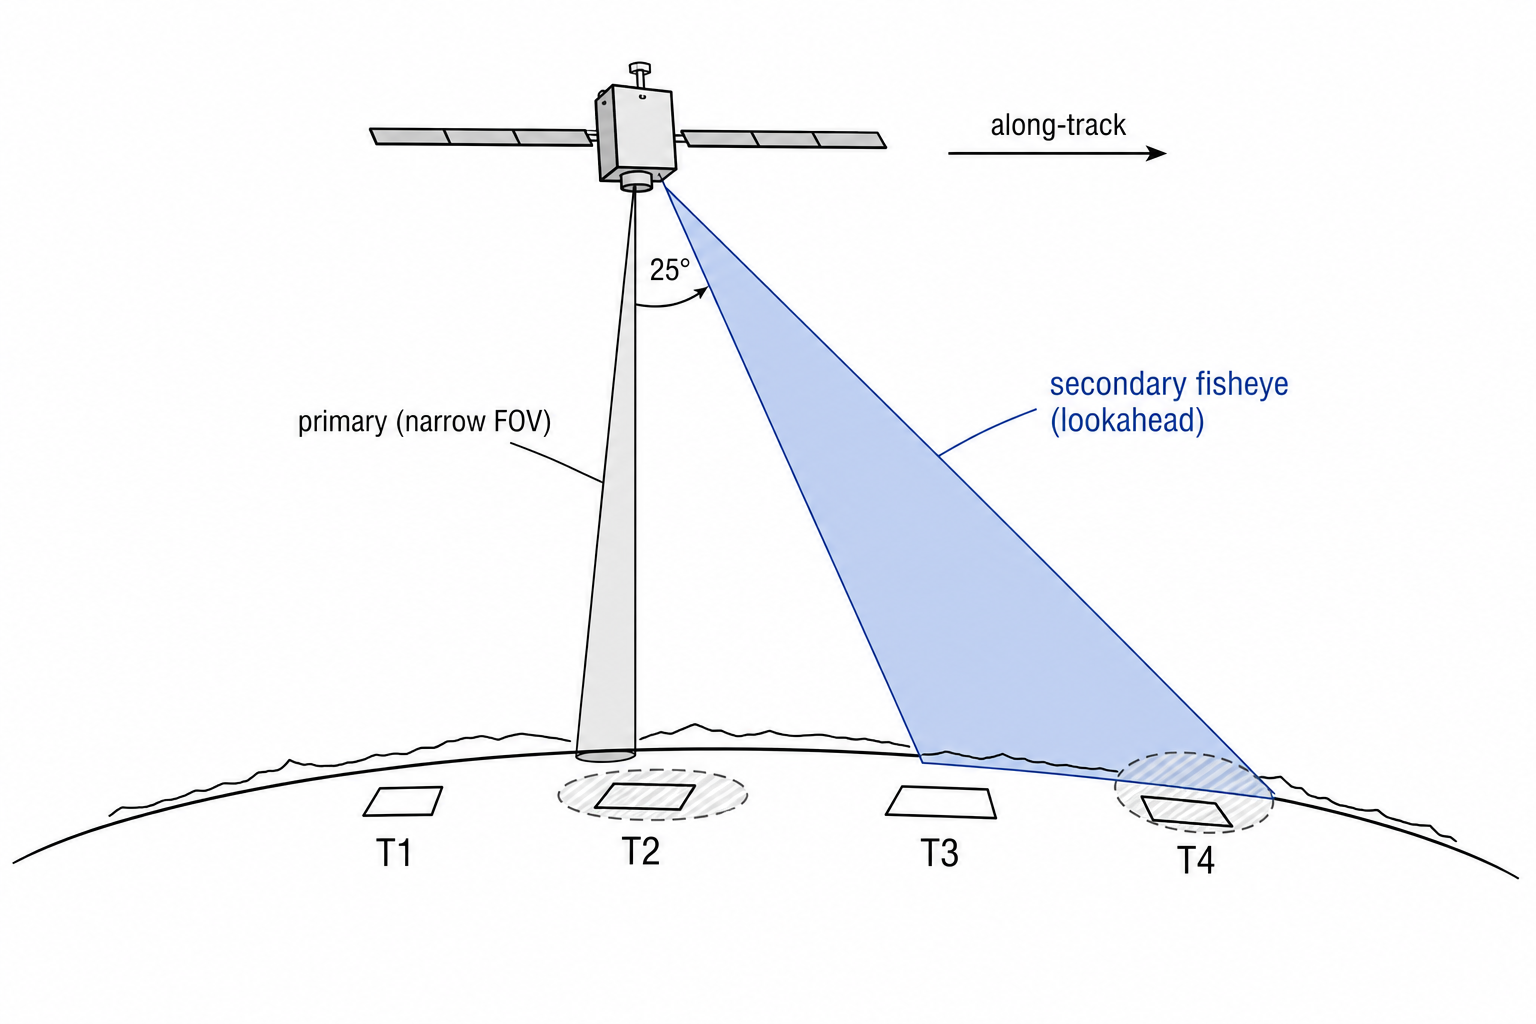
\includegraphics[width=0.92\linewidth]{figures/fig_concept_lookahead_eth.png}
  \caption{Lookahead sensing geometry.
    The narrow primary camera images near nadir while a forward-tilted fisheye observes upcoming targets along-track before they enter the primary footprint
    ($\SI{25}{\degree}$ prograde tilt; Table~\ref{tab:constants-camera-sim}).}
  \label{fig:concept-lookahead}
\end{figure}

Lookahead sensing is not unique to a fisheye.
Alternatives include cloud or weather products from other satellites, relayed via the ground segment or cross-link, and those products need not be image-shaped at all.
We evaluate the onboard fisheye approach because it is deployment-feasible on a single spacecraft and avoids network effects and external data dependencies:
as long as the satellite has power and a downlink path for the science data it produces, the scheduling loop can operate from its own sensors.

The intended decision process is sequential opportunity selection under scarcity.
The fisheye reveals clear and cloud-occluded candidates ahead of the primary footprint; an onboard policy ranks those imaging opportunities and spends the limited shutter budget (proxying storage, downlink capacity, and actuator effort) on high-value clear captures rather than executing a fixed pre-planned schedule.
This report then asks a narrower training question: which reward shaping and action-space designs make that selective behaviour learnable in simulation.

\subsection{Research question}
\label{sec:research-question}

Cloud-aware autonomous scheduling is an obvious improvement over fixed pre-planned capture.
The motivating question of this report is therefore not whether such a policy should exist, but how to train one in simulation:
\begin{quote}
  \textbf{What reward shaping and action-space design are sufficient for a reinforcement-learning agent to learn selective pointing and shuttering during a cloud-occluded Earth-observation pass?}
\end{quote}
Capture decisions are sequential and uncertain.
Cloud occlusion, attitude dynamics, and discrete shutter events interact over a single pass, so the design of the learning interface matters as much as the algorithm choice.
The experiments below treat this as a design-space question: which training choices make selective shuttering learnable, and which do not.

\subsection{Related work}
\label{sec:related-work}

Earth-observation satellite scheduling is a well-studied operations-research domain.
Surveys of satellite scheduling problems document how limited onboard storage, downlink, and energy constrain capture opportunities, and how waste of those resources reduces science yield \citep{ferrari2024ssp}.
Much of that literature addresses ground-segment planning over multi-orbit horizons.
The present work instead asks how a single-pass, onboard policy should decide pointing and shuttering when cloud cover is revealed only during the overflight.

Continuous-control reinforcement learning provides candidate algorithms for that onboard layer.
Soft Actor-Critic (SAC) combines off-policy sample reuse with a maximum-entropy objective, which tends to stabilise stochastic continuous control relative to brittle deterministic off-policy methods \citep{haarnoja2018sac}.
Maximum a Posteriori Policy Optimisation (MPO) frames improvement as relative-entropy-constrained policy iteration with separate trust regions on the policy mean and covariance \citep{abdolmaleki2018mpo}.
Both algorithms are used in the experiments below as interchangeable learners over a shared environment and observation stack.

Beyond the policy update, observation structure matters when sensors are heterogeneous.
Integrating state representation learning into deep RL shows that reward alone may not shape a usable embedding when modalities must be fused, and that structured encoders improve sample efficiency and generalisation \citep{bruin2018irl}.
For tabular and numeric inputs specifically, embedding numerical features before mixing outperforms feeding raw scalars through a shallow multilayer perceptron \citep{gorishniy2022revisiting}; that motivation underlies encoder variants that compress structured bearing and mask fields before fusion with vision features.

Prior work therefore covers Earth-observation resource scheduling, stable continuous-control RL, and structured observation encoders.
It does not, however, map which reward shaping and action-space designs are sufficient for cloud-aware shuttering under hard attitude-safety constraints in this simplified Earth-observation setting.
That mapping is the focus of the present report.

\subsection{Deterministic baseline}
\label{sec:baseline-intro}

\begin{figure}[htbp]
  \centering
  \begin{subfigure}[t]{0.32\linewidth}
    \centering
    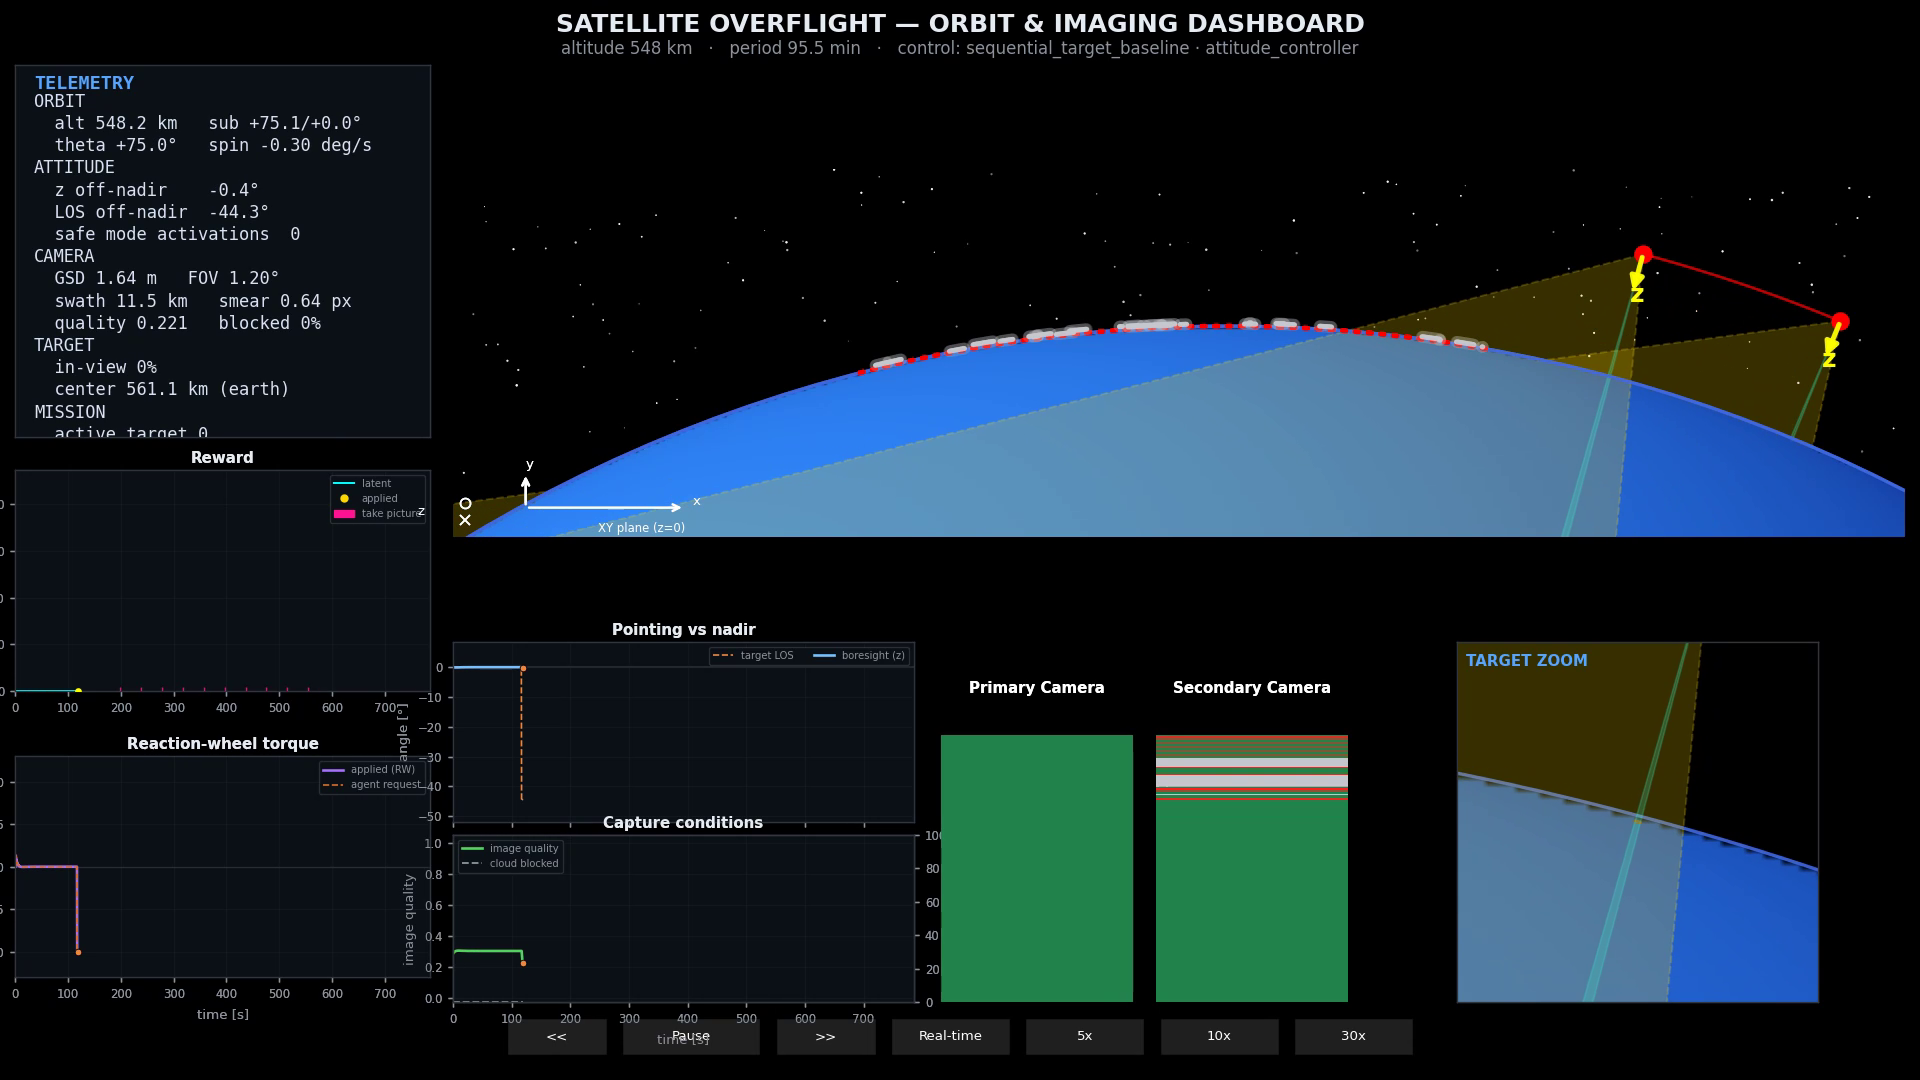
\includegraphics[width=\linewidth]{figures/fig_baseline_phase_approach.png}
    \caption{Approach}
  \end{subfigure}\hfill
  \begin{subfigure}[t]{0.32\linewidth}
    \centering
    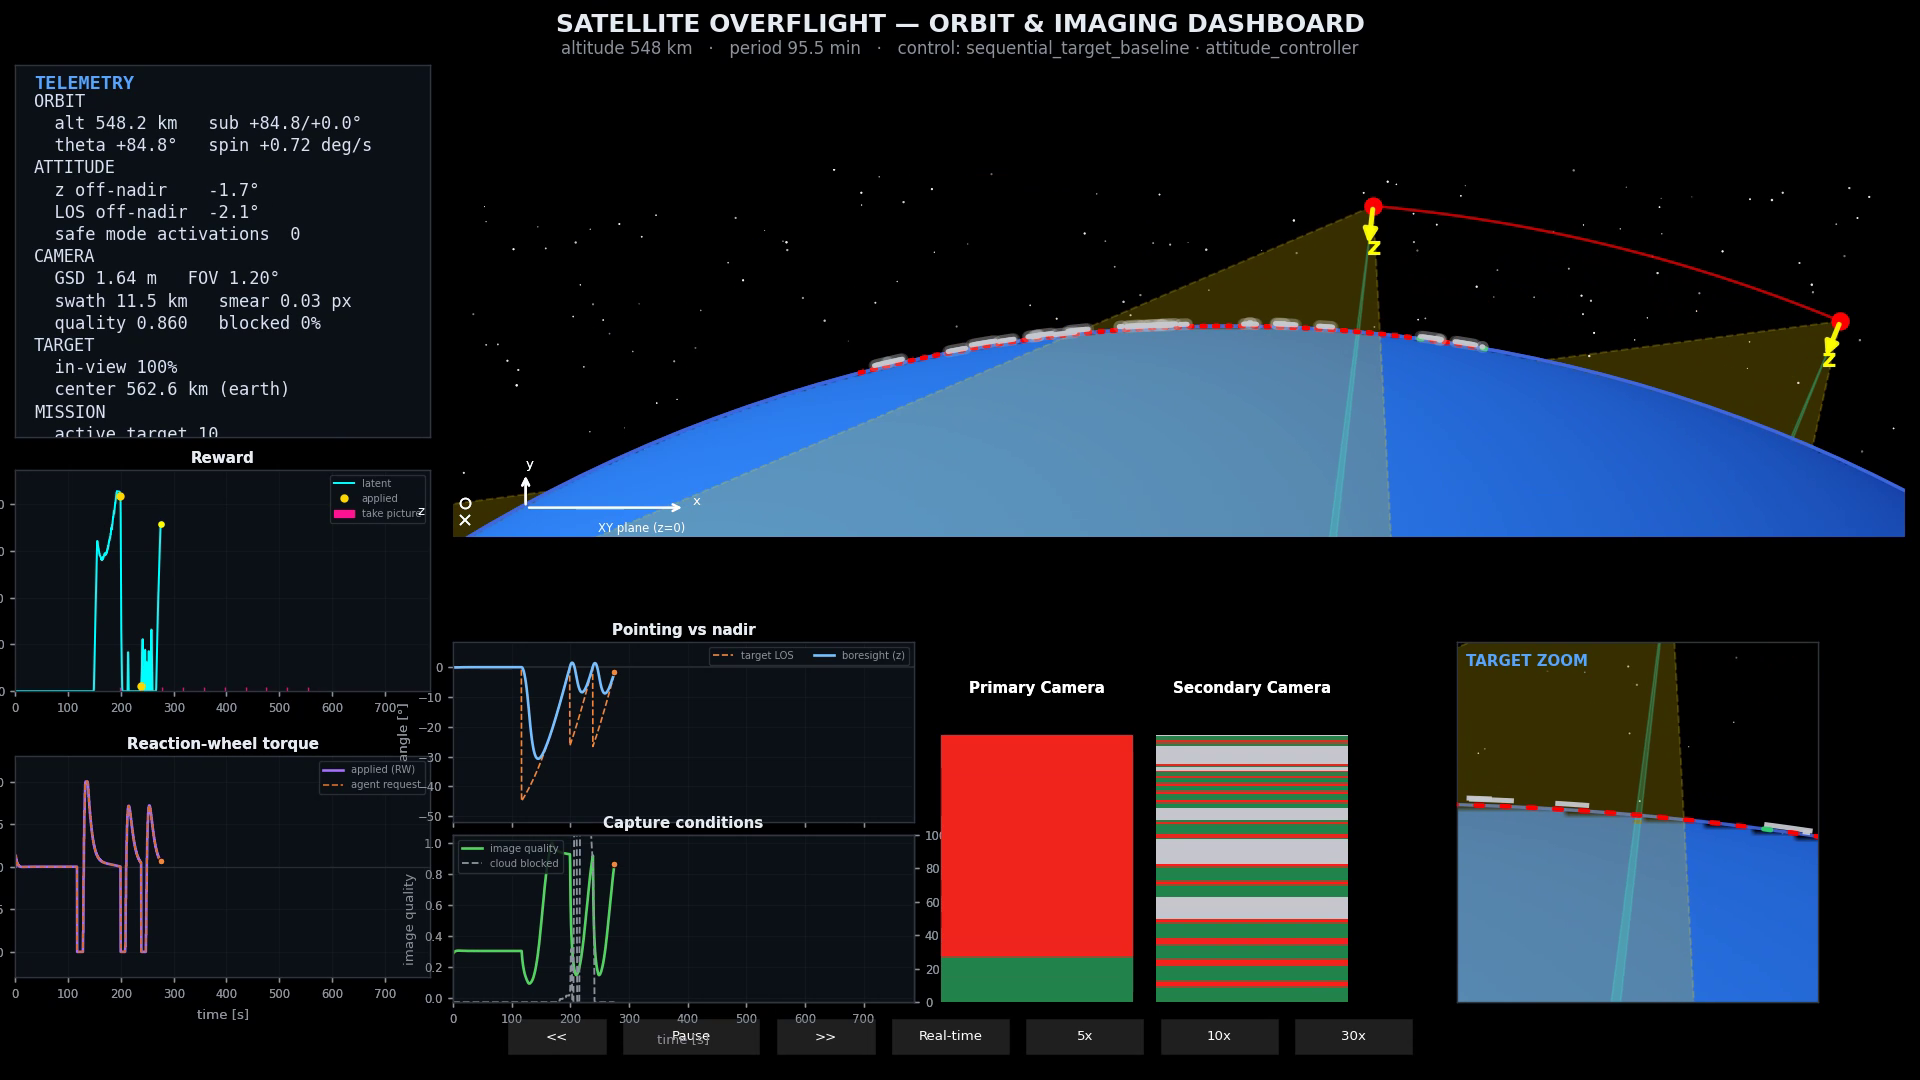
\includegraphics[width=\linewidth]{figures/fig_baseline_phase_point.png}
    \caption{Point}
  \end{subfigure}\hfill
  \begin{subfigure}[t]{0.32\linewidth}
    \centering
    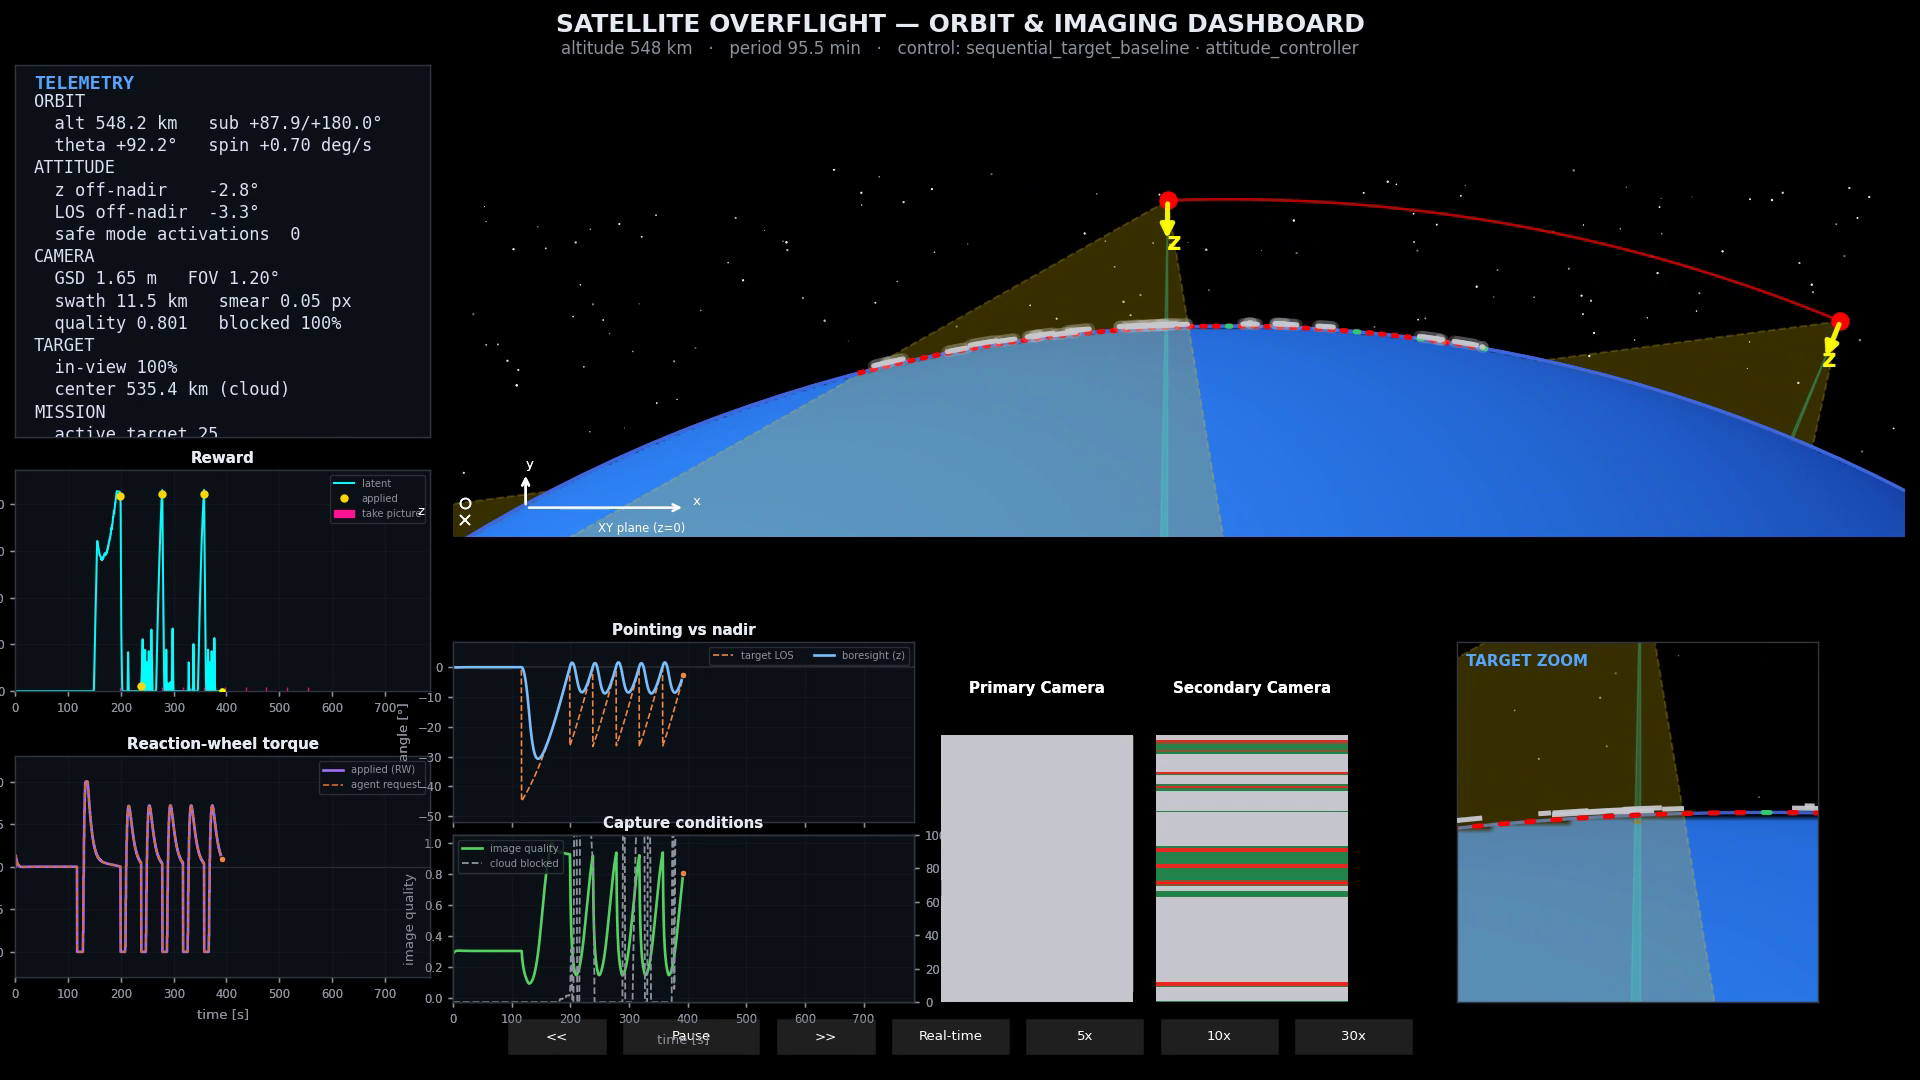
\includegraphics[width=\linewidth]{figures/fig_baseline_phase_capture.png}
    \caption{Capture}
  \end{subfigure}
  \caption{Deterministic baseline overflight (orbit-disk dashboard).
    Left to right: (a)~Approach: nadir coast into the target corridor before the first lock;
    (b)~Point: large off-nadir slew toward the scheduled target bearing;
    (c)~Capture: return to nadir after the first shutter, with high image quality and the reward spike still visible.
    The schedule fires regardless of cloud cover (Table~\ref{tab:baseline-config}).}
  \label{fig:baseline-overflight-phases}
\end{figure}

The reference strategy is a pre-scheduled sequential controller used as the comparison anchor throughout the experiments (Section~\ref{sec:baseline}): an OBC proportional--derivative loop commands target body angles (nadir coast or target bearing) under the same attitude-safety stack as the learned policy, with no cloud awareness and no adaptive capture list (see Table~\ref{tab:baseline-config}).

A real mission is additionally constrained by onboard memory, downlink bandwidth, and energy \citep{ferrari2024ssp}.
We model this resource limit with a \emph{shutter budget}: a hard cap of ten capture actions per episode.
Because the deterministic baseline treats every scheduled target equally, that budget is consumed indiscriminately across clear and cloud-occluded targets alike.
This yields a fixed, predictable observation cadence but wastes capture capacity on frames that are scientifically unusable when a cloud is in the field of view.

\subsection{Scope and simplifications}
\label{sec:scope}

The model deliberately stays close to the control problem while omitting much operational detail: 2D attitude dynamics, basic circular-orbit geometry, physical ray tracing for cameras and clouds, safety arbitration, and single-pass episodes.
It does not model multi-orbit scheduling, flight hardware, or real imagery ingestion.
Illumination conditions are not modelled: all episodes are treated as daytime passes with perfect solar lighting.
This is a deliberate simplification.
Optical Earth observation is not performed at night, and solar geometry only excludes certain orbit geometries rather than driving frame-to-frame image quality during a pass.
Cloud occlusion is a far stronger and more variable image quality constraint within a single pass, and is the focus of this work.
Section~\ref{sec:methods} describes how the question was investigated and lists modelled subsystems explicitly; Discussion states extensions (three-dimensional attitude, richer terrain, stronger RL benchmarks) as logical next steps rather than deliverables of this semester project.

\textbf{Long-term context.}
The intended onboard stack is hierarchical: a mission planner sets observation intent, a learned policy decides when and what to image, and an OBC executes maneuvers through PD pointing under hard attitude-safety limits.
This report maps the learning interface for that scheduling layer, not the full flight stack.
Section~\ref{sec:discussion-architecture} details the control hierarchy and the torque-to-vector action-interface path explored in the experiments.

\subsection{Contributions}
This report documents:
\begin{itemize}
  \item \textbf{Platform.} A simulation-and-learning pipeline with seeded mission randomisation and matched baseline comparison, so that reward and action-space variants are tested under identical cloud and target draws.
  \item \textbf{Design-space study.} A sequence of fourteen experiments that maps which reward terms, action representations, and algorithm choices enable cloud-aware shuttering behaviour, and which do not.
  \item \textbf{Evaluation protocol.} Training and evaluation conventions with a fixed environment seed, baseline-policy buffer seeding, and a deterministic baseline as the comparison anchor.
  \item \textbf{Evidence.} Qualitative and quantitative artefacts from frozen runs, including selective shuttering behaviour in late-training episodes where learning succeeded.
\end{itemize}

The engineering platform and the experimental map are the primary deliverables; mission-level outperformance of the baseline was not established within the semester scope (Section~\ref{sec:discussion}).

\subsection{Report structure}
Section~\ref{sec:solution-concept} states the intended onboard sensing and scheduling concept.
Section~\ref{sec:related-work} situates the work against Earth-observation scheduling surveys and continuous-control reinforcement learning.
Section~\ref{sec:methods} describes the research approach, simulation environment, and learning method.
Section~\ref{sec:experiments} documents the design-space search: which reward and action-space choices were tested and what each revealed.
Section~\ref{sec:results} aggregates the behavioural and return outcomes.
Sections~\ref{sec:discussion} and~\ref{sec:conclusion} interpret the mapped design space, rejected shortcuts, and outlook.
Technical constants are listed in the Nomenclature section; source-code entry points are in the Appendix.
